\documentclass[12pt]{article}

%% preamble: Keep it clean; only include those you need
\usepackage{amsmath}
\usepackage[margin = 1in]{geometry}
\usepackage{graphicx}
\usepackage{booktabs}
\usepackage{natbib}

% highlighting hyper links
\usepackage[colorlinks=true, citecolor=blue]{hyperref}


%% meta data

\title{Has Taylor Swift Succumbed? An Analysis of the Repetitive Nature of Pop Music and Its Influence on Major Musical Artists}
\author{Emma Graebner\\
  Department of Statistics\\
  University of Connecticut
}

\begin{document}
\maketitle

\begin{abstract}
The world of Pop music is dominated by few artists. One of those being the Grammy award winning country, pop, and indie folk singer Taylor Swift. Swift's influence on mainstream Pop music has been record-breaking. This article will analyze one song chosen at random from each of her ten studio albums (not including her re-released "(Taylor's Version")) for its proportion of unique words to total words. The data suggests that her Pop albums were the most repetitive, while her Indie Folk and Country albums were the least repetitive. The argument will be made that the songs that Top the Billboard 100 charts are more likely to be repetitive, and Swift has reflected that ideal in her own writing. This article will also analyze related artist's - Lady Gaga, Sam Smith, and Dua Lipa - popular works to compare with Swift's.   
\end{abstract}


\section{Introduction}
\label{sec:intro}

Are Taylor Swift’s albums the same lyrical complexity? As Taylor Swift has grown as an artist, have her albums increased in proportion of non repeated words per song? What does this say about mainstream music in relation to popular artists? How do other popular artists’ works compare to her lyrical prose? 

	Because Evermore is her “most unique” album (lyrically), what does that say about the style of music she expected to be popular during the time of conception, i.e. during the Covid pandemic of 2020? The pandemic may have played a role in what she produced for her audience. Taylor Swift' demographic is teen girls who "have grown up alongside her and her music, meaning that while no longer tween-aged, their long-term fandom is embedded with nostalgia of their own girlhoods. In addition, Swift constantly evokes these feelings to court adult fans eager to return to their younger years.” \citep{rossman2022taylor}. She used her platform to create a different style of music, one that implemented prose that tended to not repeat as much as her pop material does.
	
	This may be indicative of the Covid pandemic and the collective lonlieness the world felt -- being stuck at home, not permitted to leave unless absolutely necessary might have played into Taylor Swift's heart wrenching albums that materialized during this time. Folklore and Evermore departed from her turn to grunge pop that was seen in her 2017 album Reputation. Songs like Look What You Made Me Do, End Game, and ...Ready For It entice the listener with a new type of style. Pop music with a hint of grit in her words and melodies are exemplified in Reputation. Even the cover of the album speaks to a darker side of Taylor Swift. 


	\begin{figure}[tbp]
  \centering
  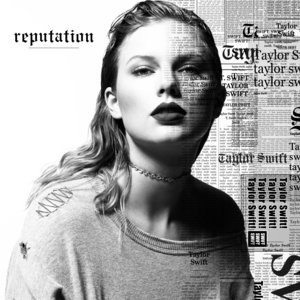
\includegraphics[width=50mm]{reputationcover}
  \caption{This is my fourth figure.}
  \label{fig:Reputation Album Cover}
\end{figure}

	\begin{figure}[tbp]
  \centering
  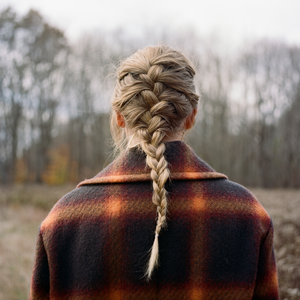
\includegraphics[width=50mm]{evermore}
  \caption{This is my fourth figure.}
  \label{fig:Evermore Album Cover}
\end{figure}

This cover compared with her next album, Folklore, showcase two very distinctly different aspects of Swift's mindset. One is more contrastive and darker (Reputation) and depicts Taylor Swift looking directly in the camera with a fierce expression. This may appeal to audiences more, like pop music, because of its enticing look. Like the Reputation album cover, Evermore shows Taylor Swift herself, but from behind. This cover appears softer in color and overall depiction. Taylor Swift is looking peacefully into the woods, away from the camera in order to give herself dimension. Though the audience looking at the photo is focusing on Taylor, she herself is focusing on the woods in the distance. This represents a departure from her previous era of pop, and into a new time of acoustic, alternative, and indie music. The unique quality of Evermore tells us that Taylor Swift might have spent more time developing the lyrics to her songs on the album. 

The unique factor of Evermore, compared to Reputation, is that Swift knows her audience, and was able to capitalize on the softer side of her work. 
	
	Other albums that came out the same year as Evermore include Chromatica by Lady Gaga and Future Nostalgia by Dua Lipa. I will analyze, at random, one song from each album to determine the uniqueness of those songs, lyrically. Comparing the complexity of those two songs (“Cool” from Future Nostalgia, and “1000 Doves” from Chromatica), I will determine how Taylor Swift’s prose is different from Lady Gaga’s and Dua Lipa’s. Similarly to Swift, Lady Gaga and Dua Lipa contributed to their respective albums by writing on every song. 
	
	Taylor Swift is the most popular artist in the country right now. Her most recent album, Midnights secured every place in the Billboard Top 10 the week of November 5th, 2022, and to this day (November 14th, 2022), her single, Anti-Hero is still at #1. To compare with another song of similar relevance on the charts today, I will analyze the proportion of unique words to total words of Sam Smith's song, Unholy. This will test how her song, Labyrinth, relates to Unholy by its lyrical prose. 

  The topic of mainstream pop music is one of contention and intrigue. Stardom is the state or status of being a famous or exceptionally talented performer in the world of entertainment (cite Oxford dictionary at some point). The conversation of an artist's ability to produce lasting and iconic materials begins with the history of an artist themselves. 
  
  Taylor Swift grew up in Reading, Pennsylvania in 1989. She had talent as a young singer, and moved to Nashville at the early age of 14 to pursue her dream of being a performer. She released her first single in 2006 (with The Big Machine record company), "Tim McGraw". She utilized social media platforms like Twitter, MySpace, Facebook, and Tumblr to promote her music. She went on to produce and release her next album Fearless in 2008, along with the various singles and music videos that proceeded. Her country albums grew in popularity, and were topping the charts for numerous weeks during this era. \cite{perone2017word}.
  
  She went on to create her albums, typically one every two years was normal for Swift. She wrote songs for other artists. In one instance, she did not reveal herself to be the author of "Better Man", written for Little Big Town, until two weeks had passed the release date. "At the core of Taylor Swift's work as a singer-songwriter, however, is a keen awareness of and talent for creating memorable and commercially appealing melodic and lyrical hooks" \citep{perone2017word}. She knows that her audience is looking to sing along with her, memorize the words to their favorite songs, and let the songs resonate with themselves. 
  
  Swift's transition from country to pop, her earlier albums having much more influence from country music, marked an increase in sales of her records. Her album 1989, the first certified pop album that Swift released, had multiple singles in the top 10 Billboard charts, and the album's singles were on repeated on the radio, for everyone to ingest. 
  
  Taylor Swift's influence on music is astounding. In 2013, after her album Red was released, "she became the first artist since The Beatles to spend
  six or more weeks at number one with three consecutive albums" \citep{newkey2014taylor}.
  
The literature has analyzed Swift's choice of words thoroughly. Her lyrics use figurative language in new and novel ways. She describes love and loss and her evocative emotional word choice paints pictures in the listeners head. Margaret Rossman writes that, "Taylor Swift has chosen to use emotional rhetoric to transpose her aura into a desire for the tangible. Swift brings fans along with her on a journey into her own past, reigniting interest in earlier forms of media and capitalizing on a tween ideal of bedroom culture" \citep{rossman2022taylor}. She knows that her demographic is one that is vulnerable to influence. She uses this to her advantage in writing her songs; the idea that she may leave a lasting impact on a growing mind is what has made her so inexplicably popular.

Though Taylor Swift's influence transcends all who top the charts in modern popular music, there is a slight unsavory aspect to her fantastical impact. Gromkowska, in an article titled, "Pop culture icons and idols. Taylor Swift and Barbie as body and identity icons for the youth" writes this:

"Another problem is related to the role of teenage music in the construction of identity among
the youth. Music is definitely one of the most important elements of their everyday life, both
as regards individuals and generations. Its significance is in most cases much bigger than
participation in school life or good exam results. For young people, music is wonderful pleasure, and the fact that they can make thousands of independent decisions regarding music
is very important to them – even if for adults these choices are banal or worthless. Besides,
participation in music creates a sense of belonging to an important community." \citep{gromkowskapop}.

This is an important idea in today's day and age of autonomy of body, mind, and spirit. Youths being in charge of their own person -- the actions they take, their identity, and how they communicate with other people -- is what makes modern day life so irrevocable.  In an article titled, "Are You Ready For It? Re-evaluating Taylor Swift", Fogarty writes "Taylor Swift is both a monument to the past and a modern megalith, toppling the music industries through her appeal to people that historically and culturally have been told that their musical tastes are invalid (like Country fans and teenage girls)" \citep{fogarty2021you}. At a time when seemingly every choice is laid out for them, choosing what music a young person listens to allows them to take control of at least one aspect of their life. That is why Taylor Swift's influence is so crucial to the development of young people, and why this topic is so relevant to today. 

SongSim is a tool that displays word repetition in a piece of music, poetry, prose, etc. The figures below describe the repetition in the most unique song that was chosen - Champagne Problems - versus the most repetitive - Labyrinth. The program uses "self-similarity matrices to visualize patterns of repetition in text. The cell at position (x, y) is filled in if the xth and yth words of the song are the same" \citep{morris2017songsim}. That is, if a words repeats in the song, a black dot is placed in the position it repeats. You can see that Labyrinth visually shows repetition more clearly than Champagne Problems. 

	\begin{figure}[tbp]
  \centering
  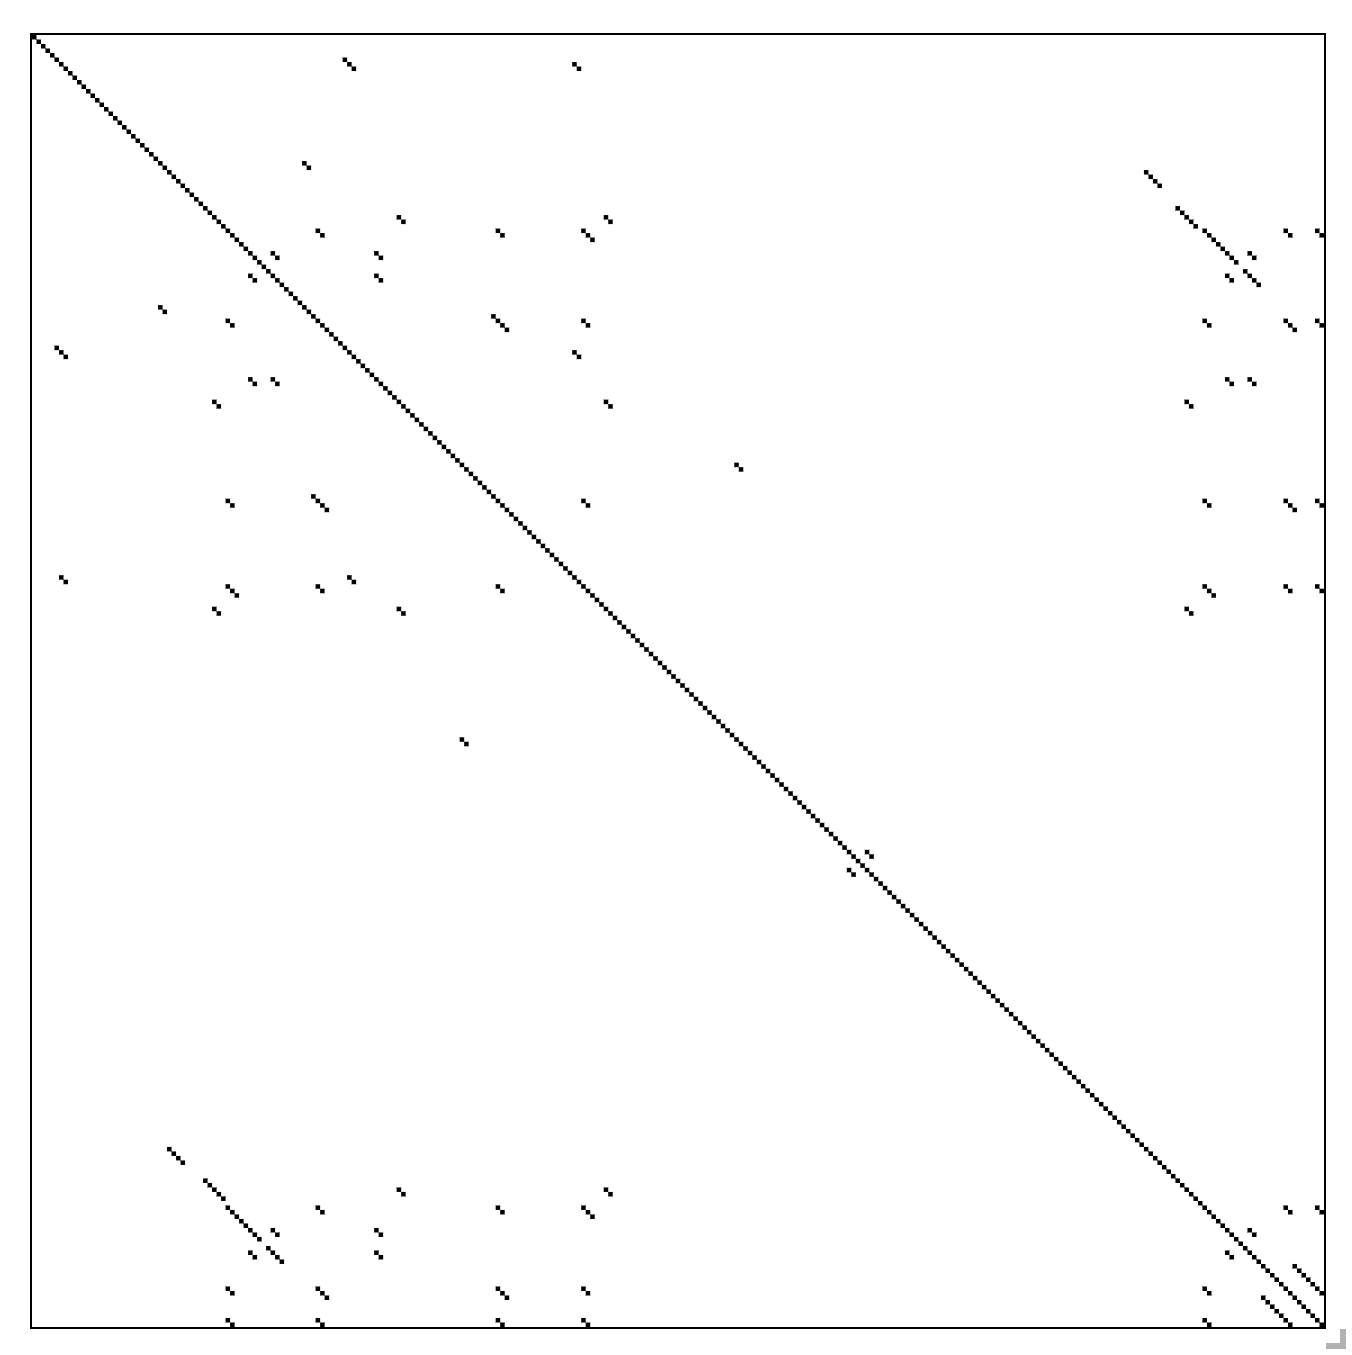
\includegraphics[width=50mm]{Champagne Problems}
  \caption{This is my fifth figure.}
  \label{fig:SongSim for Champagne Problems}
\end{figure}

	\begin{figure}[tbp]
  \centering
  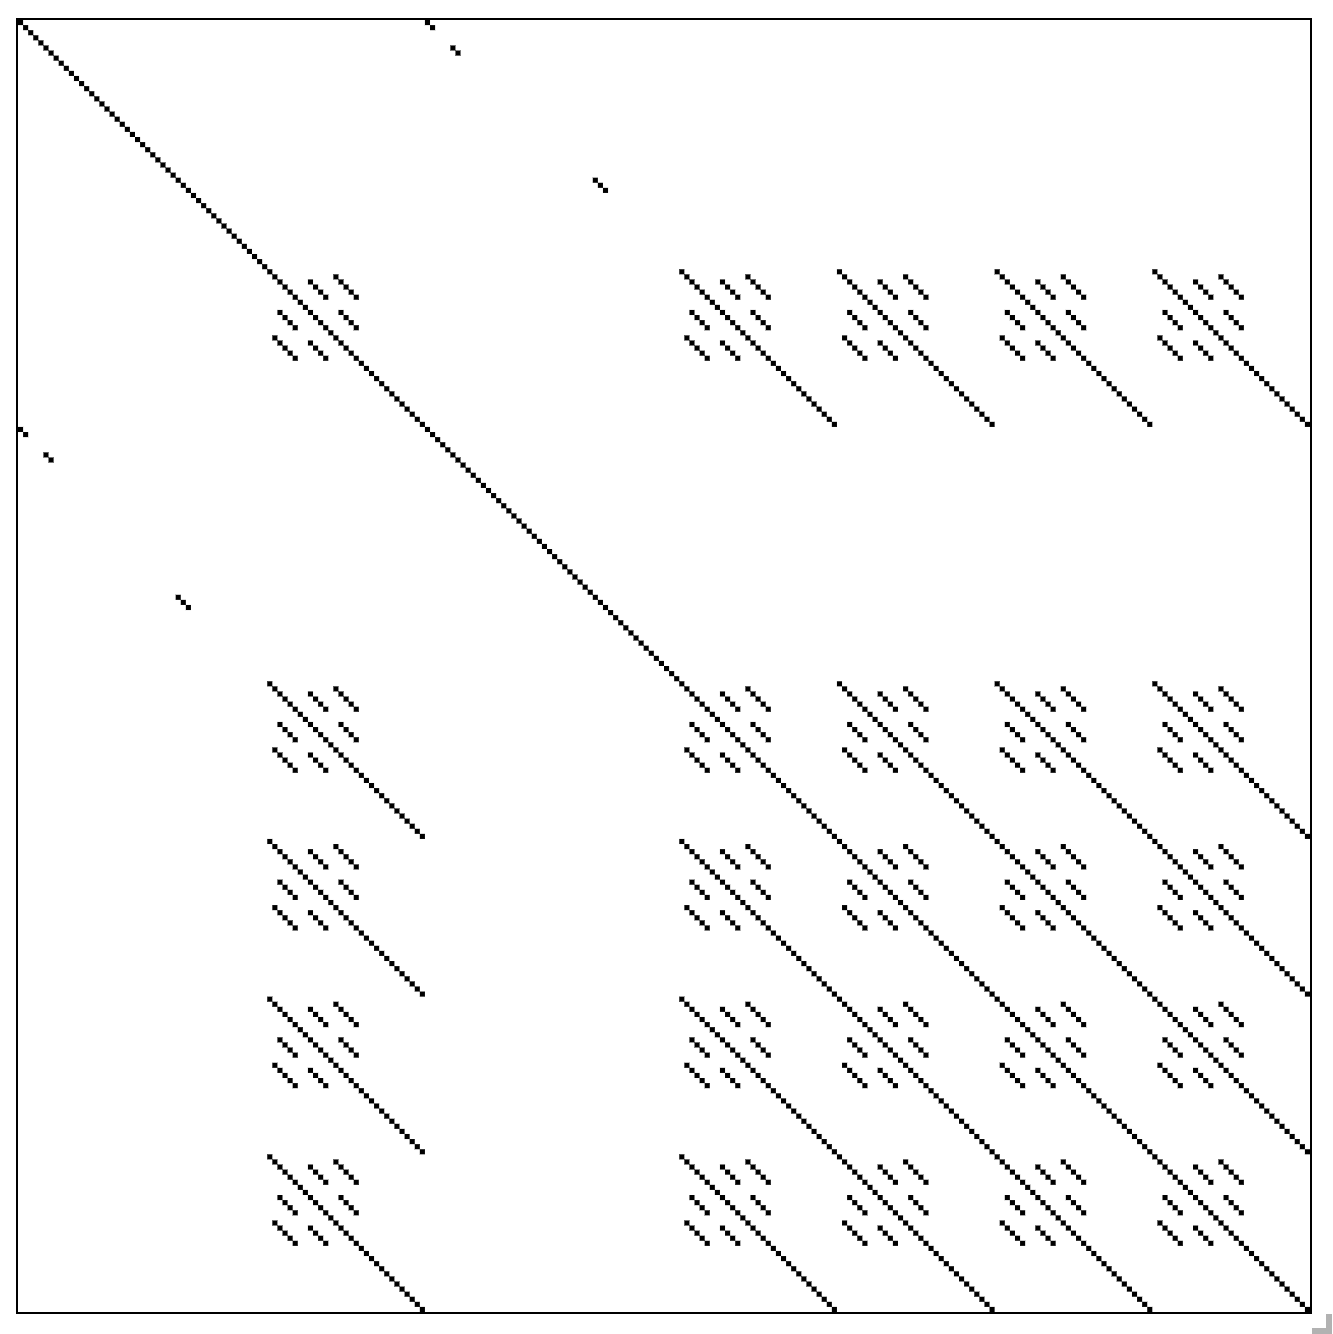
\includegraphics[width=50mm]{Labyrinth}
  \caption{This is my sixth figure.}
  \label{fig:SongSim for Labyrinth}
\end{figure}

My contribution to the work that has already been done is a method of determining how unique a song is by the proportion of unrepeated lyrics in the entire song. I will do this by putting all of the text in a spreadsheet, analyzing the text for words that do not repeat in the song, and counting them. The proportion of unrepeated words to total words is what I will be comparing amongst albums.
I will also analyze the genre change of Swift's albums: from Country to Pop to Indie Folk, then again Pop. This genre change in combination with the percentage of 


% roadmap
The rest of the paper is organized as follows.
The data will be presented in Section~\ref{sec:data}.
The methods are described in Section~\ref{sec:meth}.
The results are reported in Section~\ref{sec:resu}.
A discussion concludes in Section~\ref{sec:disc}.


\section{Data}
\label{sec:data}

The data that I am using to analyze the songs I have chosen at random is the individual work's lyrics. The software program Excel allowed me to organize my data in a readable format. It also provided a randomizer - the command "=randbetween(range)" - to chose each song from each album. I first found each song's lyrics on the acclaimed website azlyrics.com, formatted the words to be in one column, then pasted them into excel. Using the find and replace function, I got rid of any spaces. 

From there, I sorted the lyrics starting from A all the way to Z. This way, I was able to see all the repetitions of lyrics in one place. I then went through and manually searched for words that did not repeat, and assigned them a value of 1 in the column next to the word. After that was complete, I selected the column and it reported the sum (the number of ones I had put for each unique word). Then, I compared this number to the total number of words in the song; that is how the proportion of non repeated words was calculated.



\begin{table}[tbp]
  \caption{This table comprises the proportion of unique words in each Taylor Swift song from 10 different albums along with their respective genres.}
  \label{tab:rv}
\centering
\begin{tabular}{rrrr}
  \toprule
Album & Song & Proportion Unique Words & Genre \\ 
  \midrule
Taylor Swift & Cold As You & .2204 & Country \\ 
  Fearless & White Horse & .2175 & Country \\ 
  Speak Now & Sparks Fly & .2017 & Country \\ 
  Red & I Almost Do & .1413 & Country Pop\\ 
  1989 & Welcome to New York & .1391 & Synth-Pop \\ 
  Reputation & ...Ready For It & .1396 & Pop\\ 
  Lover & London Boy & .1397 & Indie Pop \\ 
  Folklore & Peace & .2334 & Indie Folk \\ 
  Evermore & Champagne Problems & .4090 & Alternative-Indie\\ 
  Midnights & Labyrinth & .1254 & Pop\\ 
   \bottomrule
\end{tabular}
\end{table}




This data explains the trend in popular mainstream music making. As you can see from the table below, the highest proportion of unrepeated words was from Taylor Swift's album entitled Evermore. The data points from Champagne Problems, the song chosen at random to represent this album, has a proportion of 0.4090; almost 41 percent of the song is unique in its prose. Her most repetitive songs include Labyrinth (from Midnights) at a proportion of .1254, Welcome To New York (from 1989) with .1391, and ...Ready For It (from Reputation) having .1396 proportion. All three of these albums are considered pop music in some way. Her most unique album, Evermore, is not classified as pop, and instead is remarked as alternative and indie. 

This distinction demonstrates the tendency of pop to be more repetitive, and less novel. According to a research article entitled, "The power of repetition: repetitive lyrics in a song increase processing fluency and drive market success", a study shows that, "more repetitive songs lyrically are processed more fluently and thus adopted more broadly and quickly in the marketplace" \citep{Nunes2015power}. People are more likely to remember words that are repeated over and over, instead of the opposite. That is how popular music sticks around and gets embedded into a culture's norms. 

Another song that has had great success in the Billboard Hot 100 charts is a song by Sam Smith (featuring Kim Petras) called Unholy. The song has a proportion of unrepeated words that amounts to 0.2017, which is considerably low compared to Evermore's Champagne Problems. Champagne Problems was number 21 on the chart for two weeks when it debuted in 2020. Sam Smith's Unholy is currently (as of November 14th, 2022) number three on the Billboard Hot 100 chart, and has risen from 11th place from last week (the week of November 8th, 2022). This is congruent with the claim that more repetitive music is more likely to be popular. Comparing the two songs, there is a difference of 0.2073 in uniqueness. That difference is approximately double the amount of unrepeated words in Champagne Problems than Unholy. 



\begin{table}[tbp]
  \caption{This table demonstrates the comparison of proportion unique words to its musical artist, genre, and time spent on the Billboard Top 100.}
  \label{tab:rv}
\centering
\begin{tabular}{rrrr}
  \toprule
Artist & Song & Proportion Unique Words & Genre \\ 
  \midrule
Dua Lipa & Cool & .0827 & Electronic Pop \\ 
  Lady Gaga & 1000 Doves  & .1764 & Electronic Pop \\ 
  Sam Smith & Unholy & .2017 & Dance Pop \\ 
  The Weeknd & Blinding Lights & .1760 & Electronic \\ 
     \bottomrule
\end{tabular}
\end{table}

\begin{figure}[htbp]
  \centering
  \includegraphics[width=\textwidth]{graph 2.png}
  \caption{This is my second figure.}
  \label{fig:graph 2}
\end{figure}

\begin{figure}[htbp]
  \centering
  \includegraphics[width=\textwidth]{graph.png}
  \caption{This is my first figure.}
  \label{fig:graph}
\end{figure}



\section{Methods}
\label{sec:meth}

Methodologies that will be generated to analyze the results of this are the use of the SongSim software that uses the repeated words of a song to express that song in a readable format. Also, I will be using the Excel formula "=randbetween(range)" to find the songs to be analyzed. The methods I used are the power of analysis using proportions. I compared the different song's proportion of unrepeated words to describe their notability. 


\section{Results}
\label{sec:resu}
The results of this analysis show that out of all of Taylor Swift's albums, the ones that were the genre of Pop were less unique than any other genre (specifically country and indie folk were her other main genres used). One may conclude from this analysis that music that fits into the genre of Pop are more likely to be popular and trending. 



\section{Discussion}
\label{sec:disc}

The main contributions of this study include the way in which her songs are analyzed. The proportion of unique words used against total words. 

The limitations of this study are that it is difficult to do any regression analysis on the type of data that I have collected. 

It is worth pursuing in the future a way to test really whether Pop music has become generally more basic in its conception and production of lyrics. 


\bibliography{references}
\bibliographystyle{mcap}

\end{document}